\chapter[How Catalysts Find Another Route]{How Catalysts\protect\\ Find Another Route}

\begin{kaichang}
\textbf{Translator safety note:} Do not pour hydrogen peroxide onto a scrape to reproduce the opening example. It is no longer recommended for wound disinfection because it can damage cells needed for healing. See \href{https://www.poison.org/articles/hydrogen-peroxide}{Poison Control's peroxide guidance}.

Your medicine cabinet may contain a little brown bottle of hydrogen peroxide solution. Pour some onto a scrape, and a layer of white foam immediately bubbles up with a hiss. Hair salons use it to dye hair too, just at a higher concentration.

Now try two thought experiments. First, leave this bottle in a cupboard and look again six months later: it is still a clear, water-like liquid, almost unchanged. Second, cut a small piece of raw pig liver and dip it into the same solution: bubbles surge out violently, as though it were boiling.

Why does the same liquid sit quietly on its own, then go ``wild'' on touching liver? What does the liver give the hydrogen peroxide---energy? Instructions? Something else? What price does the liver itself pay: does it get ``used up''? Write down your guesses, and return to check them at the end of this chapter. The answer lies in a word that runs through industry, life, and every cell in your body: \textbf{catalyst}.
\end{kaichang}

\section{A Bottle of Slow-Acting Disinfectant}

Hydrogen peroxide solution is hydrogen peroxide (\chem{H_2O_2}) dissolved in water; the kind sold in pharmacies has a concentration of only about 3\%. A hydrogen peroxide molecule has just one more oxygen atom than a water molecule, but that extra oxygen makes the whole molecule restless: at any moment, it might split apart into water and oxygen. This change releases heat and is entirely ``downhill'' in energy terms---in the language of Chapter 28, its $\Delta G$ is negative, making it a spontaneous change that thermodynamics allows and even encourages.

But ``spontaneous'' does not mean ``fast.'' Chapter 28 stressed this repeatedly, and hydrogen peroxide is an excellent living demonstration: leave a bottle of clean hydrogen peroxide solution at room temperature for a year, and only a little will decompose. Energetically, it ``wants'' to go downhill, but a high wall stands in its way---the \textbf{activation energy} introduced in Chapter 29. To decompose, a hydrogen peroxide molecule first has to twist into an awkward, high-energy shape, the transition state. At ordinary temperatures, almost no collisions supply enough energy, so the vast majority of molecules simply stay put.

Now put that little piece of liver in. Within seconds, foam churns in the cup and its wall becomes slightly warm. Insert a glowing splint (leave this step to an adult), and it will relight---that is oxygen. You have already seen the same phenomenon: hydrogen peroxide bubbles on a wound precisely because blood and tissue contain proteins that catalyze this decomposition.

Here are a few similar events in everyday life:

\begin{itemize}[itemsep=2pt]
\item Plain rice or a steamed bun tastes sweet after prolonged chewing because amylase in saliva breaks starch down into sugars. If you hold rice in your mouth without chewing, the sweetness develops much more slowly.
\item Partway along a car's exhaust system sits an inconspicuous metal canister coated inside with precious metals such as platinum, rhodium, and palladium. Carbon monoxide and nitrogen oxides in the exhaust become carbon dioxide and nitrogen as they pass through. Without it, every car would be a mobile toxic-gas factory.
\item One kind of platinum-catalyzed lighter needs no flint: press it, and fuel gas sprays onto a platinum mesh, heating up and igniting by itself. The mesh feels intact, yet it ``lights fires'' day after day.
\item In nitrogen fertilizer plants, nitrogen and hydrogen flow over layers of iron granules and become ammonia. Without this process, the world's farmland could not feed half of today's population.
\end{itemize}

Another type of catalyst may be working on the clothes you wear every day: proteases and lipases in enzyme laundry detergents specifically break down milk, blood, and grease stains. They require warm water; boiling water deactivates them, for reasons you will understand by this chapter's end. In winter, some people carry ``platinum pocket warmers'': kerosene vapor meets a platinum catalyst and continuously oxidizes, releasing heat without an open flame. They feel pleasantly warm and can stay hot all day. From detergents to pocket warmers, catalysts have long been part of daily life, quietly doing their jobs.

All these situations share one feature: a substance makes a reaction faster while apparently not being consumed itself. Such a substance is called a \textbf{catalyst}. Before memorizing a definition, let us use a small experiment to see what ``not consumed'' means.

\begin{shiyan}
\textbf{Materials}: a small bottle of pharmacy-bought 3\% hydrogen peroxide solution; a small piece of raw pig liver (or raw potato or a pinch of yeast powder---choose one); two clear cups; a kitchen scale (optional); chopsticks.

\textbf{Procedure}: fill each cup about one-third full with hydrogen peroxide solution. Leave one as a control. Put a small piece of liver, about the size of a fingernail, into the other, hold it down with chopsticks, and observe. After ten minutes, take the liver out, rinse it, and compare its size and color with the original. If using a kitchen scale, weigh the liver before and after the reaction, blotting it dry each time.

\textbf{What to observe}: (1) The difference in bubbling rate: the control hardly bubbles, while the liver cup foams vigorously. (2) Feel the outside of the liver cup: is it warm? The heat release confirms that a reaction has occurred; the energy accounting is unchanged. (3) Has the retrieved liver become smaller? It has not been ``eaten up.''

\textbf{Safety}: use only 3\% medicinal hydrogen peroxide. Higher concentrations, such as salon or industrial products, can burn skin and must not be touched. Avoid splashing hydrogen peroxide into your eyes; gloves are advisable. The glowing-splint test involves an open flame: watch only a teacher's demonstration or a video. The liver used in the experiment is no longer edible; discard it.
\end{shiyan}

The liver was not consumed. It merely ``passed through,'' and the hydrogen peroxide changed from sluggish to impatient. How did it manage that?

\section{Not a Push, but a Different Route}

Zoom in to the molecular scale. Chapter 29 offered a picture: to become products, reactant molecules must first cross an energy mountain, whose awkward, high-energy summit is the transition state. The higher the mountain, the fewer molecules can cross and the slower the reaction. Hydrogen peroxide decomposing on its own faces quite a high mountain: its chemical bonds first have to stretch almost to breaking point. With only random collisions at room temperature, even a million or a hundred million attempts rarely produce a success.

The active ingredient in liver is a protein called \textbf{catalase}; chemistry teachers use the black powder manganese dioxide (\chem{MnO_2}) for demonstrations. Both do essentially the same job: \textbf{they do not push molecules up the mountain from behind. They point them toward another route---one divided into several stages, each with a low mountain.}

Take manganese dioxide as an example. In simplified terms, there are two steps. First, a hydrogen peroxide molecule strikes the manganese dioxide surface, where a manganese atom ``catches'' it in a temporary association. Its old bonds weaken and break in the process, producing water and highly reactive fragments attached to the surface. Second, another hydrogen peroxide molecule arrives and combines with these fragments. Oxygen atoms pair up and leave as oxygen molecules, while the manganese dioxide surface returns to its original state, ready for the next visitors.

Notice the crucial point: the catalyst is \textbf{not a bystander standing outside the action}. It really joins hands with the reactants, forming a fleeting ``intermediate,'' then gracefully withdraws at the next stage and returns unharmed to the starting point. Chemists call this a ``catalytic cycle'': enter, work, leave, enter again. A grain of manganese dioxide or a catalase molecule can repeat this cycle thousands, tens of thousands, or even hundreds of millions of times in its lifetime. That is why a pinch of powder or a tiny piece of liver can ``take care of'' a whole cup of hydrogen peroxide.

The energy diagram below illustrates this ``change of route.'' Remember: this is a human-made representation. The curves depict energy levels, not any real physical shape.

\begin{center}
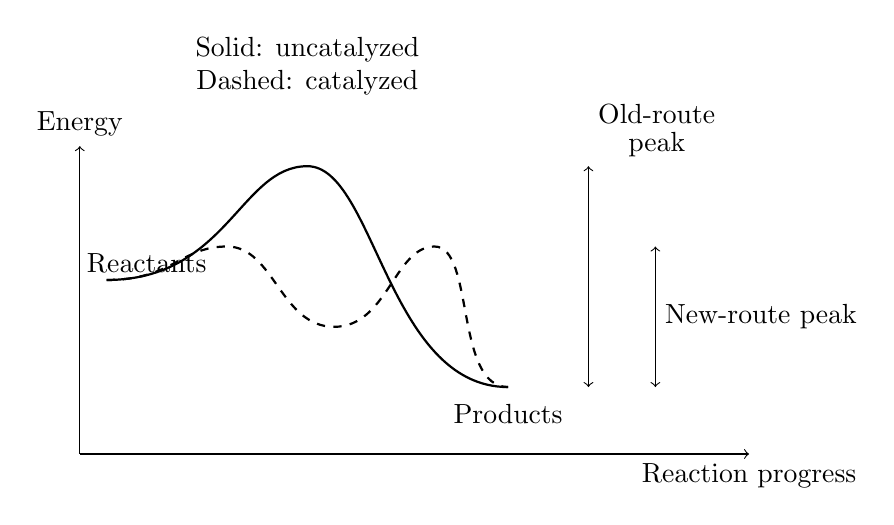
\begin{tikzpicture}[scale=0.85]
\draw[->] (0,0) -- (10,0) node[below] {Reaction progress};
\draw[->] (0,0) -- (0,4.6) node[above] {Energy};
\draw[thick] (0.4,2.6) .. controls (2.2,2.6) and (2.4,4.3) .. (3.4,4.3)
  .. controls (4.4,4.3) and (4.6,1.0) .. (6.4,1.0);
\draw[thick,dashed] (0.4,2.6) .. controls (1.4,2.6) and (1.5,3.1) .. (2.2,3.1)
  .. controls (2.9,3.1) and (3.0,1.9) .. (3.8,1.9)
  .. controls (4.6,1.9) and (4.7,3.1) .. (5.3,3.1)
  .. controls (5.9,3.1) and (5.6,1.0) .. (6.4,1.0);
\draw[<->] (7.6,1.0) -- (7.6,4.3) node[above right] {\shortstack{Old-route\\peak}};
\draw[<->] (8.6,1.0) -- (8.6,3.1) node[midway,right] {New-route peak};
\node at (1.0,2.85) {Reactants};
\node at (6.4,0.6) {Products};
\node[align=center] at (3.4,5.8) {Solid: uncatalyzed\\Dashed: catalyzed};
\end{tikzpicture}
\end{center}

The dashed route replaces one high mountain with several lower ones. Even the lowest of these is better than having no route at all: appreciable numbers of molecules can cross at ordinary temperatures, speeding the reaction up thousands or tens of thousands of times. Yet the starting point (reactants) and endpoint (products) have exactly the same heights on both routes. We will unpack this carefully in the next section, because it is a notorious trouble spot in both chemistry exams and chemistry scams worldwide.

\section{Fast and ``More'' Are Different Things}

Now let us face a particularly confusing question directly: what does a catalyst change, and what does it leave unchanged?

Start with what stays the same. Chapter 27 introduced Hess's law: a reaction's enthalpy change $\Delta H$ depends only on its starting and ending states, not its route. Whether hydrogen peroxide decomposes slowly by itself, with manganese dioxide, or with liver, the total heat released on forming water and oxygen is exactly the same. The endpoints have not changed, so not one entry in the ledger changes. Similarly, Chapter 28's $\Delta G$ depends only on initial and final states: it determines the direction and the limit, and a catalyst cannot touch it.

Then there is equilibrium. Chapter 31 will discuss chemical equilibrium in detail; for now, remember this conclusion: the position at which a reversible reaction reaches equilibrium---the proportions of reactants and products---is determined by the equilibrium constant $K$, whose value depends entirely on the energy accounting. A catalyst \textbf{changes neither the equilibrium constant nor the equilibrium position}. It does just one thing: lets the system \textbf{reach more quickly} the position already determined for it. This is because the catalyst treats forward and reverse reactions equally: a route built for the forward direction works just as well backward. Both directions speed up by the same factor, leaving their ratio, and thus the destination, unchanged.

For an analogy, put the reactants at a mountain's foot and the products in a lower valley beyond its summit. Nature has fixed the difference in elevation. Originally, the only route was a dangerous, little-used path over the main peak; a catalyst is like a new tunnel that cuts the journey from days to hours. But the tunnel cannot change the elevation difference or the fact that ``living in the valley is more comfortable.'' It merely speeds travel in both directions. During a flood, both tunnel entrances become submerged; the direction still depends on which land is lower.

\begin{qiaoliang}
How much can a catalyst accelerate a reaction? Chapter 29 gave the intuition behind the Arrhenius relation: rate is extremely sensitive to activation energy $E_a$, scaling roughly as $e^{-E_a/(RT)}$, where $R=\ud{8.314}{J\cdot mol^{-1}\cdot K^{-1}}$ and $T$ is absolute temperature. Suppose a catalyst lowers a reaction's activation energy from $\ud{75}{kJ\cdot mol^{-1}}$ to $\ud{50}{kJ\cdot mol^{-1}}$ at room temperature, $298\ \mathrm{K}$. The rate increases by a factor of
\[
\frac{k_{\text{cat}}}{k_{\text{orig}}} = e^{(75-50)\times 10^{3}/(8.314\times 298)} = e^{25000/2478} \approx e^{10.1} \approx 2.4\times 10^{4}.
\]
Shaving just $\ud{25}{kJ\cdot mol^{-1}}$ off the ``mountain''---roughly a small fraction of an ordinary covalent bond's energy---makes the reaction over twenty thousand times faster. This is why exponential functions are such powerful mathematics in chemistry: a small activation-energy difference produces orders-of-magnitude differences in speed. Catalase in liver is even more dramatic: it accelerates this decomposition by about $10^{14}$, and one enzyme molecule can process over a million hydrogen peroxide molecules per second. Hydrogen peroxide produced by your liver's daily metabolism would damage cells if not removed promptly, but a small handful of enzyme molecules breaks it into water and oxygen in seconds.
\end{qiaoliang}

\section{How Symbols Keep the Accounts}

Only now do symbols enter the picture. Catalysts have a special place in chemical equations: neither among the reactants nor among the products, but \textbf{above the arrow}, like a ``road-condition notice'':

\[\chem{2H_2O_2} \xrightarrow{\chem{MnO_2}} \chem{2H_2O} + \chem{O_2}\]

The notation itself expresses a chemist's honesty: manganese dioxide appears in neither accounting column; it is simply a condition for using this route. In your cells, catalase carries out the same reaction, written the same way:

\[\chem{2H_2O_2} \xrightarrow{\text{catalase}} \chem{2H_2O} + \chem{O_2}\]

Here are two more reactions we will meet repeatedly. First, ammonia synthesis by the Haber process (Chapter 31 will return to its equilibrium accounting):

\[\chem{N_2} + \chem{3H_2} \rightleftharpoons \chem{2NH_3}\]

Iron is the catalyst, written above the reversible arrow; note that the reaction is reversible, and iron accelerates both directions. One reaction in a car's catalytic converter is:

\[\chem{2CO} + \chem{2NO} \rightarrow \chem{2CO_2} + \chem{N_2}\]

Precious metals such as platinum and rhodium are this route's ``tunnel builders.'' Incidentally, the reaction's $\Delta G$ is already negative: when carbon monoxide and nitric oxide coexist, becoming carbon dioxide and nitrogen is energetically favorable. They can ``peacefully coexist'' all the way out through the exhaust solely because no route is available; the converter's entire job is to open that route.

\section{Three Ways to Build a Route}

Catalysts have more than one way to build routes. The common approaches fall into three categories.

\textbf{Solid-surface catalysis} (heterogeneous catalysis). Manganese dioxide, platinum mesh, and iron granules for ammonia synthesis all belong here. Reactant molecules adsorb onto the solid surface, where atoms hold, position, and bend them. Old bonds weaken under this ``pressure,'' neighboring atoms help new bonds form, and the products then desorb and leave. Since all the work happens at the surface, surface area is everything: industrial catalysts are made as porous granules or honeycombs. A gram of platinum catalyst can have an internal surface area as large as a room when spread out. This also explains why dust and grease trouble catalysts: once their surfaces are occupied, the route is ruined.

\textbf{Acid--base catalysis} (a type of homogeneous catalysis). A hydrogen ion, \chem{H^+}, is an agile ``transfer station'': it first attaches itself to an atom in the reactant, making a bond weak and easy to break; after the reaction, the hydrogen ion is released unchanged. Hydrolyzing sugar into glucose and fructose, or heating starch in dilute acid to make dextrin, both involve hydrogen ions working in cycles. Acid-catalyzed esterification in the opposite direction follows the same principle (we will meet it again in Volume II's organic chemistry).

\textbf{Enzyme catalysis}. Enzymes are precise pockets formed by folded proteins. Hundreds of millions of years of evolution have refined their shape, charge, and affinity for or aversion to water, so that they fit one kind or class of molecule and position it for the easiest transformation. Catalase, amylase, and every digestive enzyme in your gut belong here. Enzymes are efficient and highly selective, but share proteins' fragility: excessive temperature or unsuitable acidity changes the pocket's shape and stops it working. Enzymes are so fascinating and important that Chapter 49 in Volume II devotes a whole chapter to them. For now, remember one thing: enzymes \textbf{are catalysts too}, and obey all the same rules---they supply no energy and change no equilibrium, only the route.

\section{Haber's Gamble: Building a Reaction Route}

\begin{zhengju}
At the start of the twentieth century, the world faced a quiet crisis: farmland lacked nitrogen. Nitrogen is a framework element in proteins and genetic material. Four-fifths of the air is nitrogen gas, yet the three bonds in its molecules are exceptionally strong (Chapter 17 discussed this bond's strength), making it unavailable to plants. Agriculture then depended on Chilean nitrate and guano, whose reserves were visibly dwindling. Scientists calculated that unless the nitrogen fertilizer problem was solved, population growth at the time would bring widespread famine within decades.

Making ammonia from nitrogen and hydrogen is thermodynamically feasible; speed was the whole problem. Nitrogen's triple bond means an intimidatingly high activation energy. Without a catalyst, the reaction is so slow that it effectively does not exist. In 1909, the German chemist Haber used osmium and uranium catalysts at high temperature and pressure to make ammonia flow at a visible rate for the first time. But Bosch and his team at BASF made the reaction industrial. Osmium was too expensive and scarce. Bosch's assistant Mittasch undertook a task so painstaking it became great, and so great it became glorious: systematically testing tens of thousands of catalyst formulations---reportedly over twenty thousand experiments with more than three thousand candidate materials. In the end, the cheapest iron, with a few promoters, worked best.

Once this route opened, humanity could ``make bread from air.'' Today, food grown with the ammonia produced worldwide supports roughly half the global population's protein intake, while the process consumes about 1\% to 2\% of the world's energy. Chemical engineers still wrestle with catalysts to reduce that energy demand. The other side of the coin is just as real: ammonia also supplies explosives, and Haber later led research into chemical warfare. Catalysts take no side; they simply open a route. Whether it leads to fertilizer or explosives depends on the person at the wheel. Chemistry cannot make that judgment for you; you must make it yourself.
\end{zhengju}

\section{Catalysts Can Get ``Sick'' Too}

Catalysts are not perpetual-motion machines. Their own vulnerabilities have, in turn, shaped much of the industrial world.

\textbf{Poisoning}. If an impurity molecule particularly likes sticking to a catalyst's active sites and refuses to leave, it blocks the route. This is catalyst poisoning. A famous chain of consequences runs as follows: sulfur compounds poison iron catalysts for ammonia synthesis, so feed gases need thorough desulfurization; lead poisons platinum in car converters, so from the 1970s and 1980s onward, countries gradually removed lead additives from gasoline. One original driving force behind this far-reaching shift to ``unleaded'' fuel was protecting those few grams of precious metals in exhaust systems. Platinum in fuel cells is also vulnerable to carbon monoxide: traces can ``suffocate'' an electrode, one reason hydrogen fuel must be highly pure.

\textbf{Selectivity}. The same reactants often have several energetically acceptable routes available. A good catalyst must be not only fast but ``faithful,'' opening only the route to the desired product. Both one-carbon chemistry using synthesis gas and asymmetric synthesis of chiral molecules in pharmaceutical plants rely on catalyst selectivity (Chapter 44 explains why chirality matters to drug activity). Enzymes take selectivity to an extreme: catalase is devoted to hydrogen peroxide and barely touches other molecules.

\textbf{Cycling and regeneration}. Because a catalyst returns to its original state after a reaction, it can, in principle, cycle indefinitely: that is the essence of its economy. In practice, catalysts slowly sinter, accumulate carbon, and become poisoned, so factories have developed various ``regeneration'' techniques: burning off carbon deposits, chemical washing, and redispersion. In refinery fluid catalytic cracking units, catalyst particles circulate continuously between reactor and regenerator, like a moving conveyor belt: burn off the coke, regain their strength, then return to work.

\section{Where This Map Breaks Down}

Every model has boundaries. Those of catalysis are equally clear, and real scams have occurred at each one.

First, a catalyst \textbf{cannot revive a thermodynamically dead reaction}. Building a faster route is futile for a direction with positive $\Delta G$ that cannot proceed under the given conditions: traffic may bustle along the road, but neither end moves. The once-sensational ``water into oil'' farce violated precisely this rule: water contains no carbon, and the energy accounting does not balance. No ``miracle catalyst'' can turn it into gasoline. Whenever you hear that ``a catalyst made an impossible reaction happen,'' you can judge immediately: either the measurements are wrong or someone is lying.

Second, a catalyst \textbf{does not raise the yield ceiling}. It only changes how quickly equilibrium is reached. To raise ammonia yield from thirty to fifty percent, a plant must change temperature or pressure, or promptly remove ammonia, rather than switch to a more powerful catalyst. Those are matters of equilibrium, discussed in Chapter 31.

Third, a catalyst \textbf{has its own operating conditions}. Too cold, and adsorption fails; too hot, and enzymes denature, metal particles sinter and grow, and surface area collapses. Every catalyst has a comfortable ``operating window,'' one of the most demanding considerations in industrial reactor design.

\begin{wuqu}
``A catalyst does not participate in a reaction, so it undergoes no change whatsoever.'' This is half right and half wrong, and the wrong half is more widely repeated. Catalysts certainly \textbf{participate}: they adsorb reactants, form intermediates, and release themselves again; only their final total amount remains unchanged. Even ``no change whatsoever'' often fails: used platinum mesh becomes rougher, precious metals in car converters slowly migrate and cluster, and enzyme molecules have finite lifetimes, aging and losing activity. More precisely, a catalyst is unchanged \textbf{stoichiometrically}---it does not enter the overall ledger. But in \textbf{physical state and individual lifetime}, it wears down with time just as we do. It delivers speed at the price of gradual aging.
\end{wuqu}

\section{Back to That Piece of Liver}

Now you can check your guesses. Liver contains catalase, with an iron atom at the center of its active pocket---exactly the sort of work transition metals excel at, as Chapter 10 explained. A hydrogen peroxide molecule enters the pocket; the iron atom first ``takes'' an oxygen, then passes it to the next hydrogen peroxide molecule and returns to its original state. This catalytic cycle repeats over a million times per second. The bubbles are oxygen, the white foam is liquid puffed up by the bubbles, and the slight warmth is heat released by decomposition.

Was the liver ``used up''? No. If it became smaller, that was because its tissue was disturbed and damaged, not because the enzyme was consumed. The enzyme molecules remain unchanged after the reaction, ready for the next job. In fact, cooked liver no longer works well, because high temperatures unravel the protein's folded pocket. This loss of activity through a change of shape is protein denaturation, which Volume II will discuss specifically. What liver gives hydrogen peroxide is neither energy nor instructions, but a \textbf{ready-made, low-barrier, precisely laid-out route}.

Incidentally, raw potato and yeast can do the same job. Their catalase contents differ, so the vigor of their bubbling differs too. If you substituted another material in the experiment, the difference you observed was a difference in catalytic ability.

\section{This Route Leads to Life}

This chapter introduced one of chemistry's most remarkable classes of characters: ``route builders'' that leave the rules intact while exerting extraordinary control over speed within them. Without catalysts, many thermodynamically allowed reactions are so slow that they effectively do not exist; with catalysts, the gulf between ``can happen'' and ``can happen in time'' is bridged.

Life is the greatest beneficiary of this art of route building. Thousands of reactions take place simultaneously in each of your cells. Without enzymes, most would be negligibly slow at body temperature. In other words, \textbf{life is a chemical reaction network precisely coordinated by catalysis}. Why are enzymes more efficient and selective than industrial catalysts? How do cells control enzyme amounts and activities to switch reactions on or off? This thread leads into Volume II: Chapter 49 examines the molecular machine of an enzyme, and the subsequent accounts of metabolism, respiration, and photosynthesis give catalysts a role at every step. Starting next chapter, we will first add the final piece of the puzzle: once a reaction speeds up, where does it stop? That is chemical equilibrium.

\begin{tiaozhan}
Why must a catalyst that accelerates a forward reaction also accelerate the reverse reaction by the same factor? Behind this lies a profound symmetry, microscopic reversibility: forward and reverse reactions cross \textbf{the same summit}, the same transition state. Let the original forward and reverse activation energies be $E_a^{+}$ and $E_a^{-}$, with products lower than reactants by $\Delta H$. Then $E_a^{+}-E_a^{-}=\Delta H$. If a catalyst lowers the summit by $\Delta E$, both activation energies decrease by $\Delta E$, leaving their difference unchanged. The forward and reverse rates therefore increase by the same factor, $e^{\Delta E/(RT)}$, and the ratio $k^{+}/k^{-}$ stays fixed. Since the equilibrium constant $K$ is proportional to this ratio, $K$ does not change. The conclusion is clear: \textbf{any substance that speeds the approach to equilibrium necessarily leaves equilibrium itself unchanged}. This is not an empirical generalization but a necessary consequence of energy geometry. A claim to have invented a catalyst that ``accelerates only the forward reaction'' belongs in the same category as a perpetual-motion machine.
\end{tiaozhan}

\section*{Try It Yourself}

\begin{sikaoti}
\item Draw an energy diagram, with reaction progress on the horizontal axis and energy on the vertical axis, showing uncatalyzed and catalyzed routes for the same reaction. Use arrows to mark each activation energy. Which segment represents $\Delta H$? Is it the same for both routes?
\item In an ammonia plant, engineers replace the iron catalyst with a new catalyst twice as efficient. Will the \textbf{equilibrium yield} of ammonia change? How might the plant's \textbf{daily output} change? Answer in separate columns headed ``Fast'' and ``More.''
\item Someone claims to have invented a catalyst that splits water into hydrogen and oxygen at ordinary temperature and pressure with no energy input. Use the energy accounting of water electrolysis to explain why this is impossible. Where is the claimed ``hydrogen'' more likely to come from?
\item Design an experiment to test whether manganese dioxide really is ``not consumed'' during hydrogen peroxide decomposition. Hint: the insoluble black solid can be filtered, washed, dried, and weighed. What interfering factors must you also rule out?
\item Why was leaded gasoline phased out worldwide? From the perspective of catalyst poisoning, write the causal chain: lead additives $\rightarrow$ \dots $\rightarrow$ worse exhaust pollution.
\item Cooking liver greatly reduces its catalytic ability, whereas manganese dioxide remains effective after being heated red-hot. How does this difference arise from their different ``route-building tools''?
\end{sikaoti}
